\documentclass[]{article}
\usepackage{lmodern}
\usepackage{amssymb,amsmath}
\usepackage{ifxetex,ifluatex}
\usepackage{fixltx2e} % provides \textsubscript
\ifnum 0\ifxetex 1\fi\ifluatex 1\fi=0 % if pdftex
  \usepackage[T1]{fontenc}
  \usepackage[utf8]{inputenc}
\else % if luatex or xelatex
  \ifxetex
    \usepackage{mathspec}
  \else
    \usepackage{fontspec}
  \fi
  \defaultfontfeatures{Ligatures=TeX,Scale=MatchLowercase}
\fi
% use upquote if available, for straight quotes in verbatim environments
\IfFileExists{upquote.sty}{\usepackage{upquote}}{}
% use microtype if available
\IfFileExists{microtype.sty}{%
\usepackage{microtype}
\UseMicrotypeSet[protrusion]{basicmath} % disable protrusion for tt fonts
}{}
\usepackage[margin=1in]{geometry}
\usepackage{hyperref}
\hypersetup{unicode=true,
            pdftitle={manuscript},
            pdfauthor={Yuanning Li},
            pdfborder={0 0 0},
            breaklinks=true}
\urlstyle{same}  % don't use monospace font for urls
\usepackage{graphicx,grffile}
\makeatletter
\def\maxwidth{\ifdim\Gin@nat@width>\linewidth\linewidth\else\Gin@nat@width\fi}
\def\maxheight{\ifdim\Gin@nat@height>\textheight\textheight\else\Gin@nat@height\fi}
\makeatother
% Scale images if necessary, so that they will not overflow the page
% margins by default, and it is still possible to overwrite the defaults
% using explicit options in \includegraphics[width, height, ...]{}
\setkeys{Gin}{width=\maxwidth,height=\maxheight,keepaspectratio}
\IfFileExists{parskip.sty}{%
\usepackage{parskip}
}{% else
\setlength{\parindent}{0pt}
\setlength{\parskip}{6pt plus 2pt minus 1pt}
}
\setlength{\emergencystretch}{3em}  % prevent overfull lines
\providecommand{\tightlist}{%
  \setlength{\itemsep}{0pt}\setlength{\parskip}{0pt}}
\setcounter{secnumdepth}{0}
% Redefines (sub)paragraphs to behave more like sections
\ifx\paragraph\undefined\else
\let\oldparagraph\paragraph
\renewcommand{\paragraph}[1]{\oldparagraph{#1}\mbox{}}
\fi
\ifx\subparagraph\undefined\else
\let\oldsubparagraph\subparagraph
\renewcommand{\subparagraph}[1]{\oldsubparagraph{#1}\mbox{}}
\fi

%%% Use protect on footnotes to avoid problems with footnotes in titles
\let\rmarkdownfootnote\footnote%
\def\footnote{\protect\rmarkdownfootnote}

%%% Change title format to be more compact
\usepackage{titling}

% Create subtitle command for use in maketitle
\newcommand{\subtitle}[1]{
  \posttitle{
    \begin{center}\large#1\end{center}
    }
}

\setlength{\droptitle}{-2em}

  \title{manuscript}
    \pretitle{\vspace{\droptitle}\centering\huge}
  \posttitle{\par}
    \author{Yuanning Li}
    \preauthor{\centering\large\emph}
  \postauthor{\par}
      \predate{\centering\large\emph}
  \postdate{\par}
    \date{10/17/2018}


\begin{document}
\maketitle

\hypertarget{lamellibrachia-genome}{%
\section{Lamellibrachia genome}\label{lamellibrachia-genome}}

\hypertarget{abstract}{%
\subsection{Abstract}\label{abstract}}

\hypertarget{introduction}{%
\subsection{Introduction}\label{introduction}}

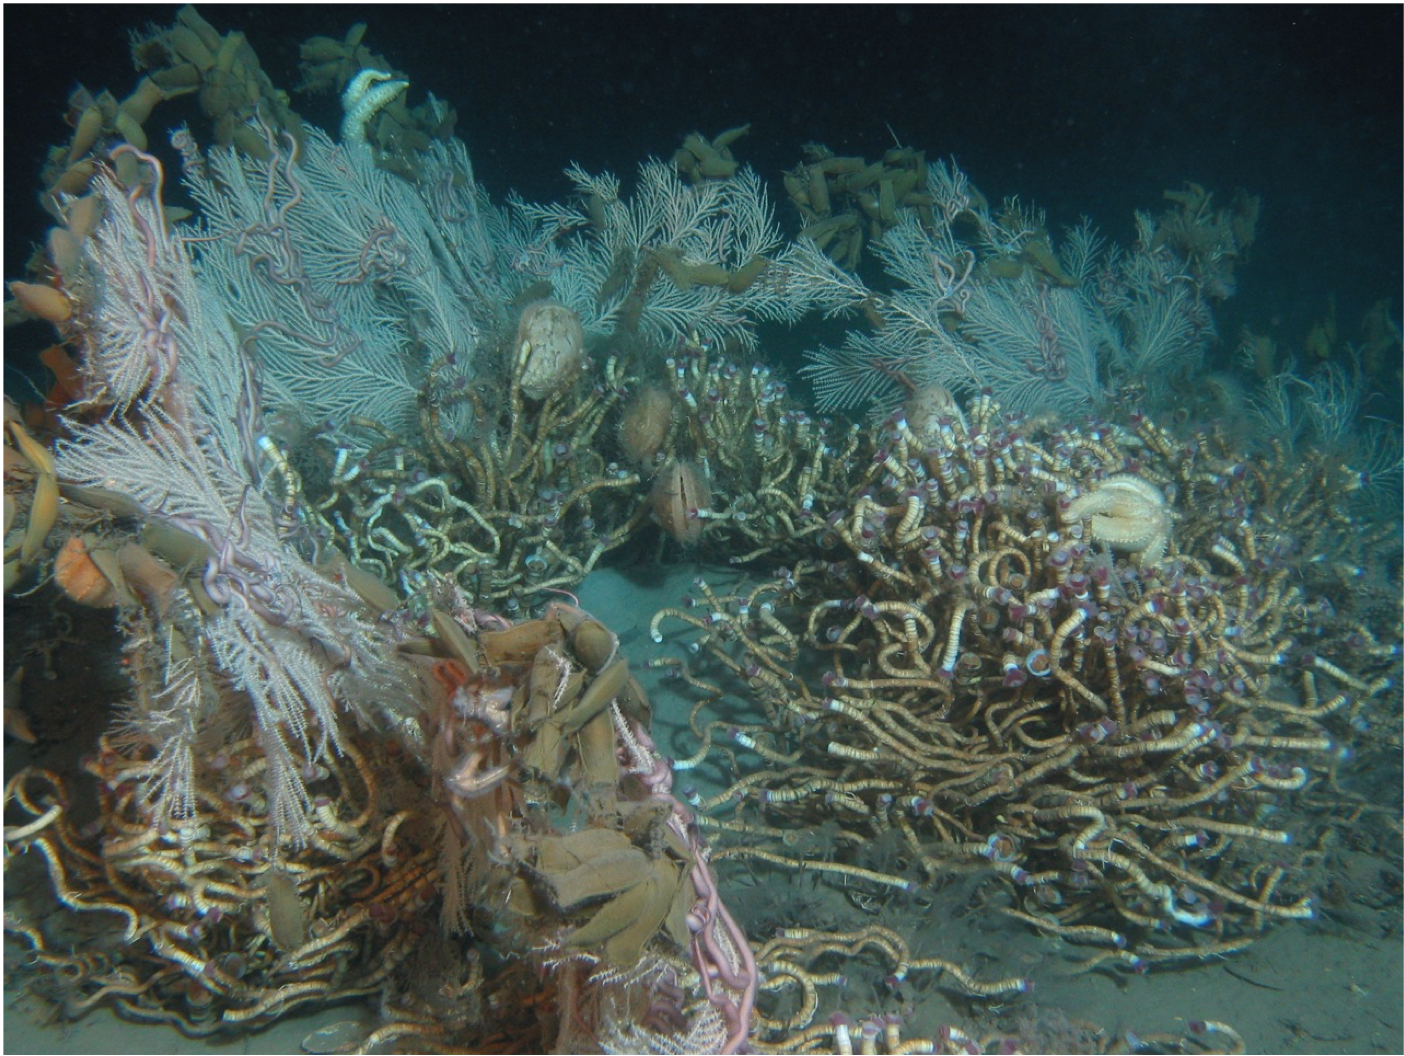
\includegraphics{../figures/Picture1.png} \textbf{Fig 1.}
\emph{Lamellibrachia} from seep localities in Gulf of Mexico.

Considerabel debate persists concenring the evolutionary origins of
siboglinids, owing to conflicting theories of its origins from fossil
and molecular age estimates. Siboglinids have been claimed to be as old
as 430 MYA based on fossil tubes found in the Silurian fossil vent
communities (Little 2002), but molecular clock analyses suggest a much
recent ( 50-126MYA) origin based on COI or 16S sequences (Little and
Vrijenhoek 2003). Recently, Late Cretaceous \emph{Osedax} fossil traces
on reptile falls provides a firm calibration point for the molecular
clock of the siboglinids (\textasciitilde{}100MYA) (Danise and Higgs
2015). Moreover, a detailed chemical and morphological analyses of tubes
from the Figueroa deposits were made by vestimentiferans, which greatly
extends the age of this lineage than previous molecular clock analyses
(Georgieva et al. 2017).

\hypertarget{methods}{%
\subsection{Methods}\label{methods}}

Scripts and data for the analyses are available in a git repository at
\url{https://github.com/yzl0084/Lamellibrachia-genome}.

\hypertarget{biological-materials.}{%
\subsubsection{Biological materials.}\label{biological-materials.}}

Adult \emph{Lamellibrachia} \emph{luymesi} specimens were collected from
seep localities in the Mississippi Canyon at 754 m depth in Gulf of
Mexico (N 28°11.58', W 89°47.94'), using the R/V Seward Johnson and
Johnson Sea Link in October 2009. All samples were frozen at 80˚C
following collection.

\hypertarget{genome-sequencing-and-assembly.}{%
\subsubsection{Genome sequencing and
assembly.}\label{genome-sequencing-and-assembly.}}

Vestimentum tissue was dissected from one individual of worm, and high
molecular weight genomic DNA was extracted using the DNeasy Blood \&
Tissue Kit (Qiagen) according to the manufacturer's protocols.
Sequencing a total of six paired-end or mate-pair genomic DNA libraries
with insert sizes ranging from 180 bp to 7 kb were performed by The
Genomic Services Lab at the Hudson Alpha Institute in Huntsville,
Alabama on an Illumina HiSeq 2000 platform (see details in Table S1).
Paired-end libraries (180 bp, 400 bp, 750 bp) were prepared using the
125 bp TrueSeq protocols, and mate-pair libraries (3-5 kbp, 5-7 kbp)
were generated using the Illumina Nextera Mate Pair Library Kit followed
by size selection. Moreover, a 10X sequencing library was constructed
using the 10X Chromium protocol (10X genomics) at the Hudson Alpha
Institute. The finished library was sequenced on an Illumina HiSeqX
platform, using paired 151 bp reads with a single 8 bp index read.

Our workflow of genome assembly was shown in Fig. S1. Two The paired-end
and 10X raw reads were checked using FastQC v0.11.5 (Andrews and others
2010) and quality filtered (Q score \textgreater{}30) using Trimmomatic
v0.36 (Bolger, Lohse, and Usadel 2014). The estimation of genome size,
level of heterozygosity and repeat contes of the Lamellibrachia genome
was determined by analaysing the kmer histograms generated from the
paired-end libraries using Jellyfish v2.2.3 (Marçais and Kingsford 2011)
and GenomeScope (Vurture et al. 2017) (Fig. S2). The Mate-pair reads
were trimmed and sorted using NxTrim v0.3.1 (O'Connell et al. 2015)
which can recgonize and trim the artificial Nextera mate-pair
circulation adapters. Only reads from category ``mp'' (true mate-pair
reads) and ``unkonwn'' (mostly large insert size reads) were used for
downstream scaffolding anlaysis. Reads from ``pe'' (paired-end reads)
and ``se'' (single ends) categories were discarded.

Given that high heterozygosity of \emph{Lamellibrachia} genome, all
reads were assembled using Platanus v1.2.4 (Kajitani et al. 2014) with a
kmer size of 32. Scaffolding was conducted by mapping Illumina
paired-end and mate-pair reads to contigs genrated by Platanus using
SSPACE v3.0 (Boetzer and Pirovano 2014). Gaps in the scaffolds were then
filled with GapCloser v1.12 (Luo et al. 2012). Redundant allele scaffods
were further remvoed using Redundans v0.13c with default settings
(Pryszcz and Gabaldón 2016). Genome assembly quality was assessed using
QUAST v3.1 (Gurevich et al. 2013). Completeness of obtained genome was
assessed using BUSCO v3(Waterhouse et al. 2017) with Metazoa\_odb9
database (978 busco genes).

\hypertarget{transcripome-assembly-and-analysis}{%
\subsubsection{Transcripome assembly and
analysis}\label{transcripome-assembly-and-analysis}}

Total RNA was extracted from the plume, vestimentum and trophosome
tissue from the same indivdisual of \emph{Lamellibrachia} spicemen using
Trizol. RNA-seq of adult tissues from plume, vestimentum and trophosome
was performed using Illumina HiSeq 2000 platform in Hudson Alpha. After
quality checking and trimming of raw sequencing reads, transcripts were
assembled de novo with Trinity. Transcript isoforms with high similarity
(≥ 95\%) were removed with CD-HIT-EST v4.7 (Li and Godzik 2006).
Transcript abundance was estimated with Bowtie v2.2.9 (Langmead and
Salzberg 2012) and RSEM v1.2.26 (Li and Dewey 2011) by mapping reads
back to the transcriptomic assembly based on transcripts per million
(TPM). A tissue specifically expressed gene was defined as a gene that
had over 75\% of the total transcripts in a particular tissue based on
TPM (Albertin et al. 2015). GO enrichment analysis was performed based
on the GO annotation using PANNZER2 (Törönen, Medlar, and Holm 2018).
Statistically overrepresented GO terms of trophosome-specific genes were
identifed using Lamellibrachia gene models as background with AgriGO (Du
et al. 2010).

\hypertarget{genome-annotation.}{%
\subsubsection{Genome annotation.}\label{genome-annotation.}}

Our genome annotation workflow was shown in Fig. S3. Gene models of
\emph{Lamellibrachia} genome were constructed following the Funannotate
pipeline 1.3.0 (\url{https://github.com/nextgenusfs/funannotate}).
Briefly, repeptive regions in the \emph{Lamellibrachia} genome were
identified usning RepeatModeler v1.0.8 (Smit and Hubley 2008) and were
subsequently soft-masked using RepeatMasker v4.0.6 (Chen 2004). RNA-Seq
data from different tissue were leveraged to improve the accuracy of
gene prediction. RNA-Seq data were assembled \emph{de} \emph{novo} into
transcriptomes using Trinity v2.4.0 (Haas et al. 2013) and HISAT 2.1.0
(Kim, Langmead, and Salzberg 2015) was used to algin RNA-Seq reads to
the \emph{Lamellibrachia} assembly. Transcrptome assemblies were then
passed to PASA pipeline v2.3.3 (Haas et al. 2003) to identify high
quality gene models. The aligned RNA-Seq data wes used to train the
\emph{ab} \emph{initio} gene predictions using AUGUSTUS v3.3 (Stanke et
al. 2006). Protein alignements from the SwissProt database to
``Lamellibrachia'' assembly were generated using exonerate (Slater and
Birney 2005) and Trinity/PASA transcripts were aligned to the genome
using Minimap2 v2.1 (Li 2018). The tRNA genes were identified using
tRNAscan-SE v1.3.1 (Lowe and Eddy 1997). Finally, EvidenceModeler 1.1.0
(Haas et al. 2008) was used to combine all the evidences of gene
prediction from protein alignemnts, transcritp alignments, and \emph{ab}
\emph{initio} predictions to construct high quality gene models.
Finally, functional annotations of predicted gene models were analyzed
using several curated databases. KEGG orthology was assinged using the
KEGG Automatic Annotation server. Gene models were further annotated
with domain structure and protein identity by InterProScan (Zdobnov and
Apweiler 2001) and SwissProt database, respectively. Secreted proteins
were predicted using SignalP (Petersen et al. 2011) and Phobius (Käll,
Krogh, and Sonnhammer 2007) using InterProScan.

\hypertarget{phylogenomics-adn-molecular-clock-analysis}{%
\subsubsection{Phylogenomics adn Molecular clock
analysis}\label{phylogenomics-adn-molecular-clock-analysis}}

Analysis of siboglinid phylogeny was conducted from publically available
16 transcriptomic data in conjuction with \emph{Lamellibrachia}
proteome. Sequence assembly, annotation, homology evaluation, gene tree
construction, parsing of genes trees to OGs, and supermatrix
construction were conducted with Agalma (Dunn, Howison, and Zapata
2013). The final analyses presented here contained 13 siboglinids and
four outgroups based on current understanding of annelid phylogeny.
Maximum likelihood analyses were performed in IQTree under the
best-fitting models for associated partition schemes determined by
Modelfinder implemented in IQTree 1.6.3 (Nguyen et al. 2014) with
ultrafast bootstrapping of 1000 replicates.

For molecular clock analysis, a relaxed molecular clock with a lognormal
distribution and a Yule tree model was used in BEAST 2 v2.5.1 (Bouckaert
et al. 2014). A calibration was placed on the node representing the most
recent common ancestor (MRCA) of \emph{Osedax} using a normal
distribution with a mean of 100 MYA and a standard deviation of 10
following the findings of (Danise and Higgs 2015).Another calibrartion
was placed on the node of MRCA of Serpulida and Sabellida using a normal
distribution with a mean of 267 MYA (Sanfilippo et al. 2017). Molecular
clock analyses with BEAST 2 consisted of two independent runs with 1
million MCMC generations sampled every 1000 generations. Convergence was
checked and confirmed by comparing trace plots in Tracer making sure the
effective sample size of each parameter was greater than 100 and that
stationarity appeared to have been achieved. Log and tree fiels were
combined using Logcombiner. A maximum clade credibility tree with mean
heights was calculated using TreeAnnotater. The resulted time-calibrated
tree was plotted using R package, phyloch, strap and OutbreakTools.
Bayesian inference using a molecular clock resulted in identical
branching patterns as analysis with IQTree.

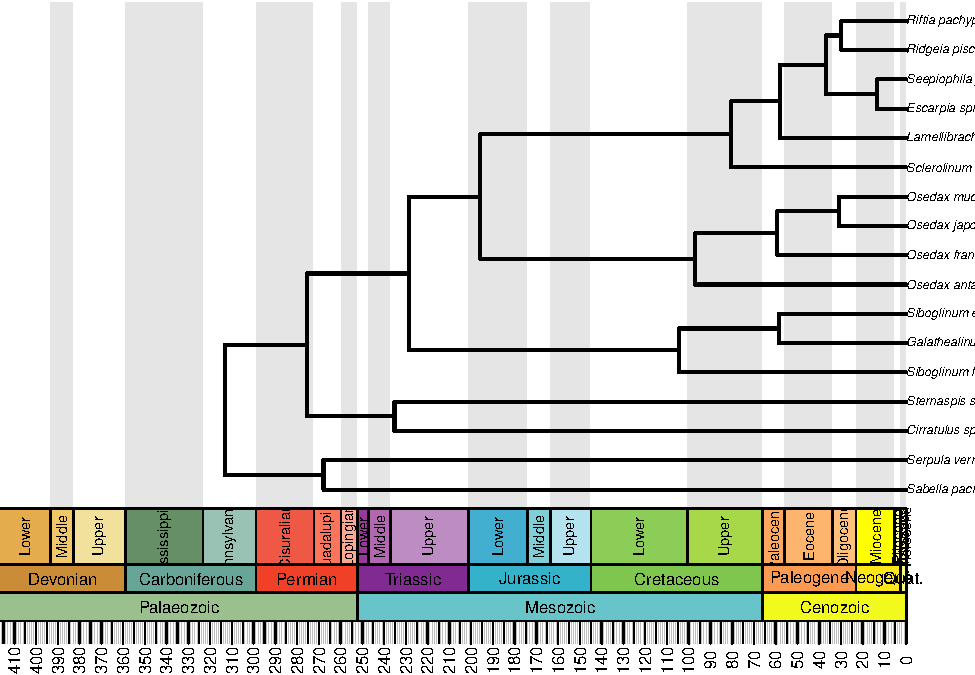
\includegraphics{manuscript_files/figure-latex/preliminaries-1.pdf}

\hypertarget{gene-family-analysis}{%
\subsubsection{Gene family analysis}\label{gene-family-analysis}}

After all-to-all Diamond v1.0 (Buchfink, Xie, and Huson 2014) BLASTP
searches against 12 selecte lophotrochozoan proteomes, orthology groups
(OGs) were identified using Orthofinder with a dfault inflation
parameter (I=1.5). Gene ontology annotation was performed using PANTHER
v13.1 (Mi et al. 2016) with the PANTHER HMM scoring tool
(pantherScore2.pl). Gene family expansion and contraction was estimated
using CAFÉ v2.1 (De Bie et al. 2006). For each gene family, CAFÉ
generated a family-wide P value, with a significant \emph{P} value
indicating a possible gene-family expansion or contraction event. A
branch-specific \emph{P} value was also generated for each branch/node
using the Viterbi method. A family-wide \emph{P} value less than 0.01
and a branch/node Viterbi \emph{P} value less than 0.001 was considered
as a signature of gene family expansion/contraction for a specific gene
family and specific species, respectively, as suggested in manual.

\hypertarget{hemoglobin-and-immunity-related-genes.}{%
\subsubsection{Hemoglobin and immunity-related
genes.}\label{hemoglobin-and-immunity-related-genes.}}

\hypertarget{results}{%
\subsection{Results}\label{results}}

\and Discussion

\hypertarget{genome-features}{%
\subsubsection{Genome features}\label{genome-features}}

Results from high-throughput sequencing and genome assembly for
\emph{Lamellibrachia} are presented in Table \# with at least 300 fold
coverage using a combination of Illumina paired-end, mate-pair and 10X
genomic sequencing with a variety of insert sizes. The haploid genome
assembly size is \textasciitilde{}687 Mb, similar to the result of
genome size estimation using GenomeScope (\textasciitilde{}646 Mb). The
N50 value of the assembled scaffolds and contigs is 373 Kb and 24 Kb,
respectively. Although N50 lengths and assembly quality of
\emph{Lamellibrachia} are comparable to those of other annelids
(e.g.~\emph{Capitella} \emph{teleta}, \emph{Hebdella} \emph{robusta}),
the overall genome completeness measured by BUSCO (\textasciitilde{}
95\%) is one of the highest among other lophotrochozoans (Table \#),
indicating the completeness of the genome assembly. With the support of
RNA-seq data from different tissue, we estimated \emph{Lamellibrachia}
genome contains 38,998 gene models. The genome also exhibit similar
level of heterozygosity (0.6\%) and repeptitive seuqences (36.92\%),
compared to other lophotrochzoan genomes (Table \#). Comparison among
three annelid genome revealed

\hypertarget{hemoglobin-evolution}{%
\subsubsection{Hemoglobin evolution}\label{hemoglobin-evolution}}

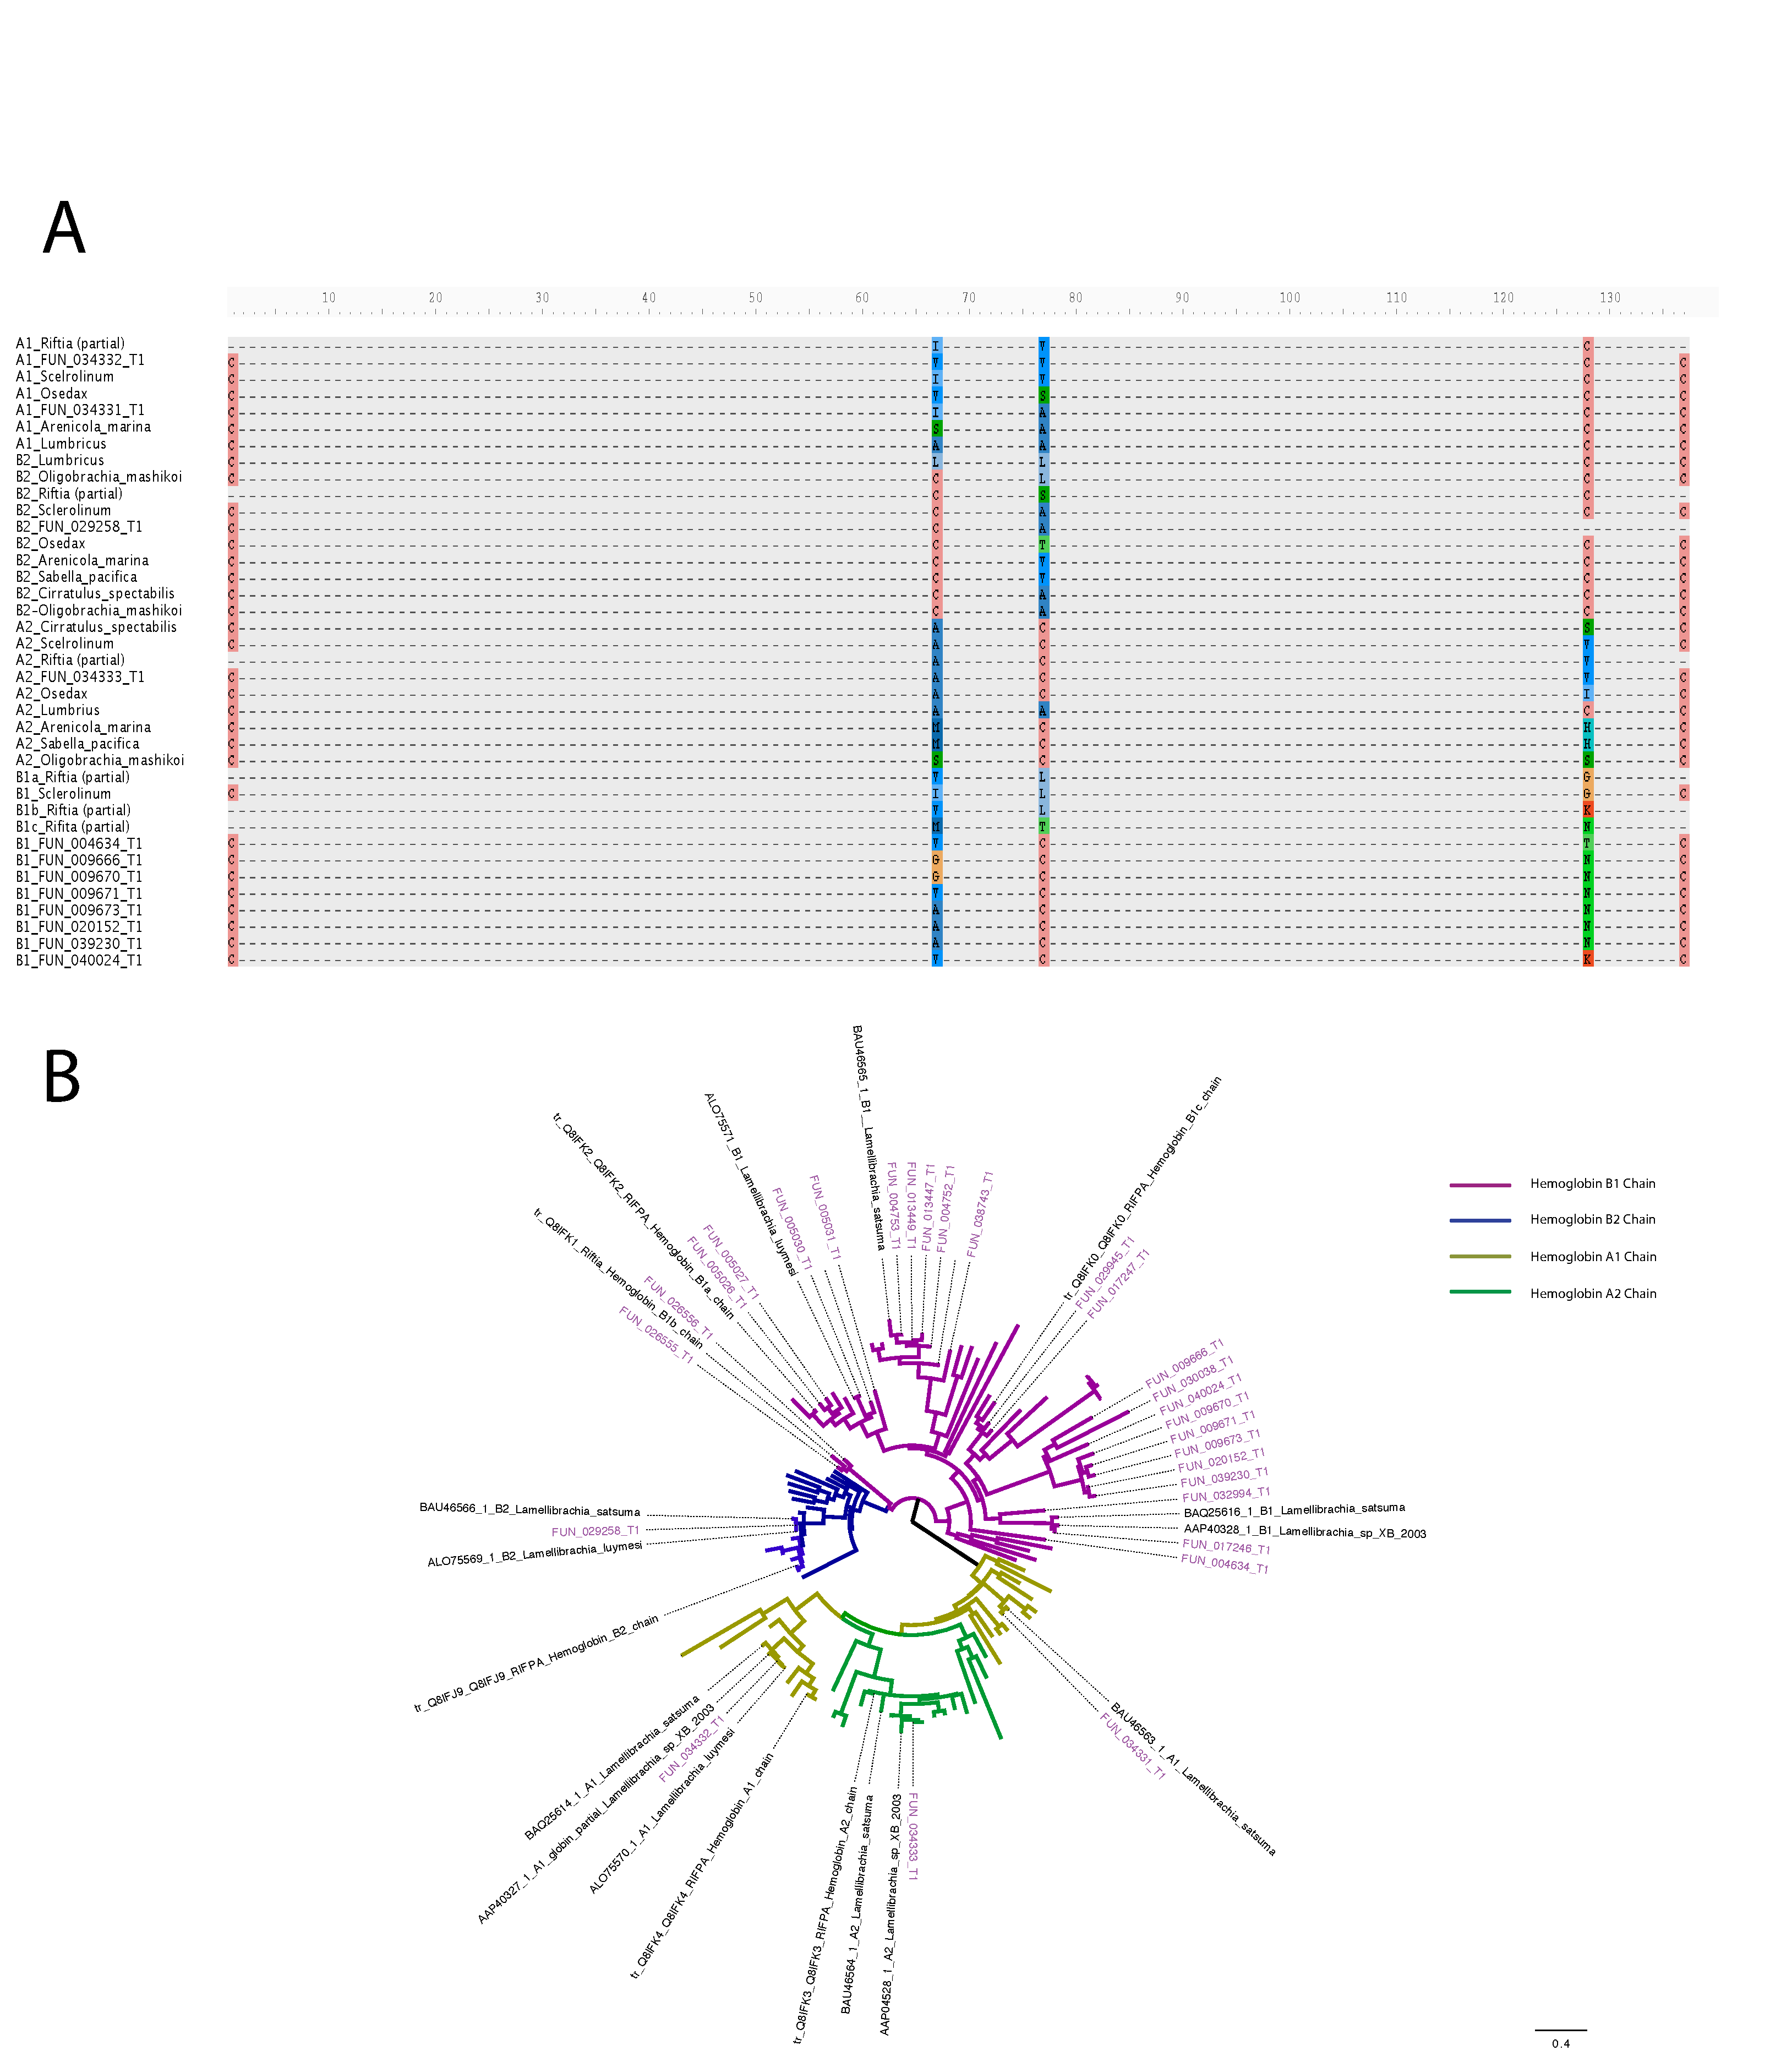
\includegraphics{../figures/hemoglobin.pdf} \textbf{Fig 2.} Hemoglobin.
Remarkably siboglinid Hbs are able to bind oxygen and sulfide
simultaneously and reversibly at two different sites. To avoid the toxic
effects of sulfide while supplying it to their chemoautotrophic
endosymbionts, siboglinds possesses a multihemoglobin system with three
different extracellular hemoglobins (Hbs; V1, V2, and C1): two dissolved
in the vascular blood, V1 and V2, and one in the coelomic fluid, C1 (Arp
and Childress 1981, @zal1996multi). Siboglinid Hbs consist of four
heme-containing chains (A1, A2, B1, B2). Sulfur-binding capabilities are
hypothesized to be due to free cysteine residues at key positions in
Hbs, especially in the A2 and B2 chains. V1 Hb can form persulfide
groups on its four linker chains, a mechanism that can account for the
higher sulfide-binding potential of this Hb (Zal et al. 1997). Moreover,
part of the H2S binding affinity has also been suggested to be mediated
by the zinc moieties bound to amino acid residues at the interface
between pairs of A2 chains in \emph{Riftia} (Flores et al. 2005).

\hypertarget{phylogeny-and-molecular-clock-of-tubeworm}{%
\subsubsection{Phylogeny and molecular clock of
tubeworm}\label{phylogeny-and-molecular-clock-of-tubeworm}}

Two additional \emph{Osedax} taxa were added in the study compared to
the previous siboglinid phylogenomic analyses (Li et al. 2017) (Table
\#). The final supermatrix dataset contains 191 genes single-copy
orthologs. Bayesian inference with a relaxed molecular clock (Fig. 2)
recovered the same topology as ML analysis in IQTree with strong nodal
support (Fig. \#). Both analyses strongly support \emph{Osedax} is most
closely related to the Vestimentifera + \emph{Sclerolinum} clade and
Frenulata is the early diverging group, as recently reported (Li et al.
2015). Within Vestimentifera, \emph{Lamellibrachia} is sister to the
remaining sampled vestimentiferans.

Molecular clock analyses based on phylogenomic dataset suggest modern
siboglinid diversity originated in Mesozoic (223MYA ± 80 MY),
conflicting with previous hypotheses indicate a Late Mesozoic or
Cenozoic approximately 50-126 MYA. The previous analyses are solely
based on estimation of nucleotide divergence of COI sequences on limited
taxa sampling (mainly vestimentiferans). However, mitochondrial genes of
vestiemntiferans may have experienced a ``slow-down'' in rate of
nucleotide subsitution relative to other siboglinid lineages (Li et al.
2015). Moreover, molecular clock analysis suggest a yonger split of
Vestimentifernas during the Cenozoic (60 MYA). Recent analyses suggested
that Jurassic tubes from Figueroa deposits is likely to have been made
by vestimentiferans (Georgieva et al. 2017), but this hypothesisis not
supported in our analysis. Thus, we provide the molecular clock of the
siboglinid phylogenetic tree, placing a common siboglinid ancestor as
far back as the Jurassic. Siboglinid vestimentifernas might exploit and
adapt to vents and seeps during Cenozoic (\textless{}65 MYA). This adds
to the growing evidence that the Cenozoic was a key period for the
radiation of most dominant invertebrate taxa now occupying in deep-sea
chomosynthetic communities (Vrijenhoek 2013).

\hypertarget{conclusion}{%
\subsection{Conclusion}\label{conclusion}}

\hypertarget{ackowledgements}{%
\subsection{Ackowledgements}\label{ackowledgements}}

\hypertarget{author-contribution}{%
\subsection{Author contribution}\label{author-contribution}}

\pagebreak

\hypertarget{supplemental-information}{%
\subsection*{Supplemental Information}\label{supplemental-information}}
\addcontentsline{toc}{subsection}{Supplemental Information}

\hypertarget{refs}{}
\leavevmode\hypertarget{ref-albertin2015octopus}{}%
Albertin, Caroline B, Oleg Simakov, Therese Mitros, Z Yan Wang, Judit R
Pungor, Eric Edsinger-Gonzales, Sydney Brenner, Clifton W Ragsdale, and
Daniel S Rokhsar. 2015. ``The Octopus Genome and the Evolution of
Cephalopod Neural and Morphological Novelties.'' \emph{Nature} 524
(7564): 220.

\leavevmode\hypertarget{ref-andrews2010fastqc}{}%
Andrews, Simon, and others. 2010. ``FastQC: A Quality Control Tool for
High Throughput Sequence Data.''

\leavevmode\hypertarget{ref-arp1981blood}{}%
Arp, Alissa J, and James J Childress. 1981. ``Blood Function in the
Hydrothermal Vent Vestimentiferan Tube Worm.'' \emph{Science} 213
(4505): 342--44.

\leavevmode\hypertarget{ref-boetzer2014sspace}{}%
Boetzer, Marten, and Walter Pirovano. 2014. ``SSPACE-Longread:
Scaffolding Bacterial Draft Genomes Using Long Read Sequence
Information.'' \emph{BMC Bioinformatics} 15 (1): 211.

\leavevmode\hypertarget{ref-bolger2014trimmomatic}{}%
Bolger, Anthony M, Marc Lohse, and Bjoern Usadel. 2014. ``Trimmomatic: A
Flexible Trimmer for Illumina Sequence Data.'' \emph{Bioinformatics} 30
(15): 2114--20.

\leavevmode\hypertarget{ref-bouckaert2014beast}{}%
Bouckaert, Remco, Joseph Heled, Denise Kühnert, Tim Vaughan, Chieh-Hsi
Wu, Dong Xie, Marc A Suchard, Andrew Rambaut, and Alexei J Drummond.
2014. ``BEAST 2: A Software Platform for Bayesian Evolutionary
Analysis.'' \emph{PLoS Computational Biology} 10 (4): e1003537.

\leavevmode\hypertarget{ref-buchfink2014fast}{}%
Buchfink, Benjamin, Chao Xie, and Daniel H Huson. 2014. ``Fast and
Sensitive Protein Alignment Using Diamond.'' \emph{Nature Methods} 12
(1): 59.

\leavevmode\hypertarget{ref-chen2004using}{}%
Chen, Nansheng. 2004. ``Using Repeatmasker to Identify Repetitive
Elements in Genomic Sequences.'' \emph{Current Protocols in
Bioinformatics} 5 (1): 4--10.

\leavevmode\hypertarget{ref-danise2015bone}{}%
Danise, Silvia, and Nicholas D Higgs. 2015. ``Bone-Eating Osedax Worms
Lived on Mesozoic Marine Reptile Deadfalls.'' \emph{Biology Letters} 11
(4): 20150072.

\leavevmode\hypertarget{ref-de2006cafe}{}%
De Bie, Tijl, Nello Cristianini, Jeffery P Demuth, and Matthew W Hahn.
2006. ``CAFE: A Computational Tool for the Study of Gene Family
Evolution.'' \emph{Bioinformatics} 22 (10): 1269--71.

\leavevmode\hypertarget{ref-du2010agrigo}{}%
Du, Zhou, Xin Zhou, Yi Ling, Zhenhai Zhang, and Zhen Su. 2010. ``AgriGO:
A Go Analysis Toolkit for the Agricultural Community.'' \emph{Nucleic
Acids Research} 38 (suppl\_2): W64--W70.

\leavevmode\hypertarget{ref-dunn2013agalma}{}%
Dunn, Casey W, Mark Howison, and Felipe Zapata. 2013. ``Agalma: An
Automated Phylogenomics Workflow.'' \emph{BMC Bioinformatics} 14 (1):
330.

\leavevmode\hypertarget{ref-flores2005sulfide}{}%
Flores, Jason F, Charles R Fisher, Susan L Carney, Brian N Green, John K
Freytag, Stephen W Schaeffer, and William E Royer. 2005. ``C.''
\emph{Proceedings of the National Academy of Sciences} 102 (8): 2713--8.

\leavevmode\hypertarget{ref-georgieva2017identification}{}%
Georgieva, Magdalena N, Crispin TS Little, Jonathan S Watson, Mark A
Sephton, Alexander D Ball, and Adrian G Glover. 2017. ``Identification
of Fossil Worm Tubes from Phanerozoic Hydrothermal Vents and Cold
Seeps.'' \emph{Journal of Systematic Palaeontology}, 1--43.

\leavevmode\hypertarget{ref-gurevich2013quast}{}%
Gurevich, Alexey, Vladislav Saveliev, Nikolay Vyahhi, and Glenn Tesler.
2013. ``QUAST: Quality Assessment Tool for Genome Assemblies.''
\emph{Bioinformatics} 29 (8): 1072--5.

\leavevmode\hypertarget{ref-haas2003improving}{}%
Haas, Brian J, Arthur L Delcher, Stephen M Mount, Jennifer R Wortman,
Smith JrRoger K, Linda I Hannick, Rama Maiti, et al. 2003. ``Improving
the Arabidopsis Genome Annotation Using Maximal Transcript Alignment
Assemblies.'' \emph{Nucleic Acids Research} 31 (19): 5654--66.

\leavevmode\hypertarget{ref-haas2013novo}{}%
Haas, Brian J, Alexie Papanicolaou, Moran Yassour, Manfred Grabherr,
Philip D Blood, Joshua Bowden, Matthew Brian Couger, et al. 2013. ``De
Novo Transcript Sequence Reconstruction from Rna-Seq Using the Trinity
Platform for Reference Generation and Analysis.'' \emph{Nature
Protocols} 8 (8): 1494.

\leavevmode\hypertarget{ref-haas2008automated}{}%
Haas, Brian J, Steven L Salzberg, Wei Zhu, Mihaela Pertea, Jonathan E
Allen, Joshua Orvis, Owen White, C Robin Buell, and Jennifer R Wortman.
2008. ``Automated Eukaryotic Gene Structure Annotation Using
Evidencemodeler and the Program to Assemble Spliced Alignments.''
\emph{Genome Biology} 9 (1): 1.

\leavevmode\hypertarget{ref-kajitani2014efficient}{}%
Kajitani, Rei, Kouta Toshimoto, Hideki Noguchi, Atsushi Toyoda,
Yoshitoshi Ogura, Miki Okuno, Mitsuru Yabana, et al. 2014. ``Efficient
de Novo Assembly of Highly Heterozygous Genomes from Whole-Genome
Shotgun Short Reads.'' \emph{Genome Research}, gr--170720.

\leavevmode\hypertarget{ref-kall2007advantages}{}%
Käll, Lukas, Anders Krogh, and Erik LL Sonnhammer. 2007. ``Advantages of
Combined Transmembrane Topology and Signal Peptide Prediction---the
Phobius Web Server.'' \emph{Nucleic Acids Research} 35 (suppl\_2):
W429--W432.

\leavevmode\hypertarget{ref-kim2015hisat}{}%
Kim, Daehwan, Ben Langmead, and Steven L Salzberg. 2015. ``HISAT: A Fast
Spliced Aligner with Low Memory Requirements.'' \emph{Nature Methods} 12
(4): 357.

\leavevmode\hypertarget{ref-langmead2012fast}{}%
Langmead, Ben, and Steven L Salzberg. 2012. ``Fast Gapped-Read Alignment
with Bowtie 2.'' \emph{Nature Methods} 9 (4): 357.

\leavevmode\hypertarget{ref-li2011rsem}{}%
Li, Bo, and Colin N Dewey. 2011. ``RSEM: Accurate Transcript
Quantification from Rna-Seq Data with or Without a Reference Genome.''
\emph{BMC Bioinformatics} 12 (1): 323.

\leavevmode\hypertarget{ref-li2018minimap2}{}%
Li, Heng. 2018. ``Minimap2: Pairwise Alignment for Nucleotide
Sequences.'' \emph{Bioinformatics} 1: 7.

\leavevmode\hypertarget{ref-li2006cd}{}%
Li, Weizhong, and Adam Godzik. 2006. ``Cd-Hit: A Fast Program for
Clustering and Comparing Large Sets of Protein or Nucleotide
Sequences.'' \emph{Bioinformatics} 22 (13): 1658--9.

\leavevmode\hypertarget{ref-li2015mitogenomics}{}%
Li, Yuanning, Kevin M Kocot, Christoffer Schander, Scott R Santos,
Daniel J Thornhill, and Kenneth M Halanych. 2015. ``Mitogenomics Reveals
Phylogeny and Repeated Motifs in Control Regions of the Deep-Sea Family
Siboglinidae (Annelida).'' \emph{Molecular Phylogenetics and Evolution}
85: 221--29.

\leavevmode\hypertarget{ref-li2017phylogenomics}{}%
Li, Yuanning, Kevin M Kocot, Nathan V Whelan, Scott R Santos, Damien S
Waits, Daniel J Thornhill, and Kenneth M Halanych. 2017. ``Phylogenomics
of Tubeworms (Siboglinidae, Annelida) and Comparative Performance of
Different Reconstruction Methods.'' \emph{Zoologica Scripta} 46 (2):
200--213.

\leavevmode\hypertarget{ref-little2002fossil}{}%
Little, Crispin TS. 2002. ``The Fossil Record of Hydrothermal Vent
Communities.'' \emph{Cahiers de Biologie Marine} 43 (3/4): 313--16.

\leavevmode\hypertarget{ref-little2003hydrothermal}{}%
Little, Crispin TS, and Robert C Vrijenhoek. 2003. ``Are Hydrothermal
Vent Animals Living Fossils?'' \emph{Trends in Ecology \& Evolution} 18
(11): 582--88.

\leavevmode\hypertarget{ref-lowe1997trnascan}{}%
Lowe, Todd M, and Sean R Eddy. 1997. ``TRNAscan-Se: A Program for
Improved Detection of Transfer Rna Genes in Genomic Sequence.''
\emph{Nucleic Acids Research} 25 (5): 955.

\leavevmode\hypertarget{ref-luo2012soapdenovo2}{}%
Luo, Ruibang, Binghang Liu, Yinlong Xie, Zhenyu Li, Weihua Huang,
Jianying Yuan, Guangzhu He, et al. 2012. ``SOAPdenovo2: An Empirically
Improved Memory-Efficient Short-Read de Novo Assembler.''
\emph{Gigascience} 1 (1): 18.

\leavevmode\hypertarget{ref-marccais2011fast}{}%
Marçais, Guillaume, and Carl Kingsford. 2011. ``A Fast, Lock-Free
Approach for Efficient Parallel Counting of Occurrences of K-Mers.''
\emph{Bioinformatics} 27 (6): 764--70.

\leavevmode\hypertarget{ref-mi2016panther}{}%
Mi, Huaiyu, Xiaosong Huang, Anushya Muruganujan, Haiming Tang, Caitlin
Mills, Diane Kang, and Paul D Thomas. 2016. ``PANTHER Version 11:
Expanded Annotation Data from Gene Ontology and Reactome Pathways, and
Data Analysis Tool Enhancements.'' \emph{Nucleic Acids Research} 45
(D1): D183--D189.

\leavevmode\hypertarget{ref-nguyen2014iq}{}%
Nguyen, Lam-Tung, Heiko A Schmidt, Arndt von Haeseler, and Bui Quang
Minh. 2014. ``IQ-Tree: A Fast and Effective Stochastic Algorithm for
Estimating Maximum-Likelihood Phylogenies.'' \emph{Molecular Biology and
Evolution} 32 (1): 268--74.

\leavevmode\hypertarget{ref-o2015nxtrim}{}%
O'Connell, Jared, Ole Schulz-Trieglaff, Emma Carlson, Matthew M Hims,
Niall A Gormley, and Anthony J Cox. 2015. ``NxTrim: Optimized Trimming
of Illumina Mate Pair Reads.'' \emph{Bioinformatics} 31 (12): 2035--7.

\leavevmode\hypertarget{ref-petersen2011signalp}{}%
Petersen, Thomas Nordahl, Søren Brunak, Gunnar von Heijne, and Henrik
Nielsen. 2011. ``SignalP 4.0: Discriminating Signal Peptides from
Transmembrane Regions.'' \emph{Nature Methods} 8 (10): 785.

\leavevmode\hypertarget{ref-pryszcz2016redundans}{}%
Pryszcz, Leszek P, and Toni Gabaldón. 2016. ``Redundans: An Assembly
Pipeline for Highly Heterozygous Genomes.'' \emph{Nucleic Acids
Research} 44 (12): e113--e113.

\leavevmode\hypertarget{ref-sanfilippo2017first}{}%
Sanfilippo, Rossana, Antonietta Rosso, Agatino Reitano, and Gianni
Insacco. 2017. ``First Record of Sabellid and Serpulid Polychaetes from
the Permian of Sicily.'' \emph{Acta Palaeontologica Polonica} 62 (1):
25--38.

\leavevmode\hypertarget{ref-slater2005automated}{}%
Slater, Guy St C, and Ewan Birney. 2005. ``Automated Generation of
Heuristics for Biological Sequence Comparison.'' \emph{BMC
Bioinformatics} 6 (1): 31.

\leavevmode\hypertarget{ref-smit2008repeatmodeler}{}%
Smit, AFA, and R Hubley. 2008. ``RepeatModeler Open-1.0.''
\emph{Available Fom Http://Www. Repeatmasker. Org}.

\leavevmode\hypertarget{ref-stanke2006augustus}{}%
Stanke, Mario, Oliver Keller, Irfan Gunduz, Alec Hayes, Stephan Waack,
and Burkhard Morgenstern. 2006. ``AUGUSTUS: Ab Initio Prediction of
Alternative Transcripts.'' \emph{Nucleic Acids Research} 34 (suppl\_2):
W435--W439.

\leavevmode\hypertarget{ref-toronen2018pannzer2}{}%
Törönen, Petri, Alan Medlar, and Liisa Holm. 2018. ``PANNZER2: A Rapid
Functional Annotation Web Server.'' \emph{Nucleic Acids Research}.

\leavevmode\hypertarget{ref-vrijenhoek2013instability}{}%
Vrijenhoek, Robert C. 2013. ``On the Instability and Evolutionary Age of
Deep-Sea Chemosynthetic Communities.'' \emph{Deep Sea Research Part II:
Topical Studies in Oceanography} 92: 189--200.

\leavevmode\hypertarget{ref-vurture2017genomescope}{}%
Vurture, Gregory W, Fritz J Sedlazeck, Maria Nattestad, Charles J
Underwood, Han Fang, James Gurtowski, and Michael C Schatz. 2017.
``GenomeScope: Fast Reference-Free Genome Profiling from Short Reads.''
\emph{Bioinformatics} 33 (14): 2202--4.

\leavevmode\hypertarget{ref-waterhouse2017busco}{}%
Waterhouse, Robert M, Mathieu Seppey, Felipe A Simão, Mosè Manni,
Panagiotis Ioannidis, Guennadi Klioutchnikov, Evgenia V Kriventseva, and
Evgeny M Zdobnov. 2017. ``BUSCO Applications from Quality Assessments to
Gene Prediction and Phylogenomics.'' \emph{Molecular Biology and
Evolution} 35 (3): 543--48.

\leavevmode\hypertarget{ref-zal1996multi}{}%
Zal, Franck, François H Lallier, Brian N Green, Serge N Vinogradov, and
André Toulmond. 1996. ``The Multi-Hemoglobin System of the Hydrothermal
Vent Tube Worm Riftia Pachyptila Ii. Complete Polypeptide Chain
Composition Investigated by Maximum Entropy Analysis of Mass Spectra.''
\emph{Journal of Biological Chemistry} 271 (15): 8875--81.

\leavevmode\hypertarget{ref-zal1997primary}{}%
Zal, F, T Suzuki, Y Kawasaki, JJ Childress, FH Lallier, and A Toulmond.
1997. ``Primary Structure of the Common Polypeptide Chain B from the
Multi-Hemoglobin System of the Hydrothermal Vent Tube Worm Riftia
Pachyptila: An Insight on the Sulfide Binding-Site.'' \emph{Proteins:
Structure, Function, and Bioinformatics} 29 (4): 562--74.

\leavevmode\hypertarget{ref-zdobnov2001interproscan}{}%
Zdobnov, Evgeni M, and Rolf Apweiler. 2001. ``InterProScan--an
Integration Platform for the Signature-Recognition Methods in
Interpro.'' \emph{Bioinformatics} 17 (9): 847--48.


\end{document}
